\subsubsection{initArduino}
Implementering af Arduino
I denne funktion opsættes og initialiseres Arduinoen. Til dette anvendes funktionen \textit{Arduino}, fra Arduino Support pakken. Som paramter til funktionen amgives port navnet og board typen (i dette system en Arduino Uno). Arduino variablen gemmes herefter i handles, som en variabel.

Herudover opsættes Arduinoens input og output i funktionen. \fxnote{Mangler beskrivelse}

Selve initialiseringen sker i et try/catch statement, hvis Arduinoen ikke kan initialiseres åbnes en dialogboks (figur: \ref{fig:initArduino}), hvor operatøren kan vælge om systemet skal forsøge at oprette forbindelse igen. 

\begin{figure}[H]
	\centering
	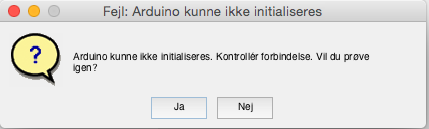
\includegraphics[width=0.5\textwidth]{billeder/software/initArduino.png}
	\caption{Dialogboks til systembesked}
	\label{fig:initArduino}
\end{figure}

Implementeringen af initArduino er vist i nedenstående kode.
\begin{lstlisting} 
while true
    % Try/Catch statement
    try
        % Initialize Arduino and save variable in handles
        handles.a = arduino('/dev/cu.usbmodem1411','Uno');
        % If succes - break while loop
        break
    catch
    % Open quest dialog to inform operator that inializing failed    
    choice = questdlg('Arduino kunne ikke initialiseres. Kontroller forbindelse. Vil du proeve igen?','Fejl: Arduino kunne ikke initialiseres', 'Ja','Nej','Ja');

        switch choice
            % Do nothing - retry inializing again
            case 'Ja'
        
            % Returns to end function
            case 'Nej'
            return
        end
    end
end
\end{lstlisting} 
